\subsection{Sugarscape}
\label{sec:sugarscape}

The seminal Sugarscape model was one of the first models in ABS, developed by Epstein and Axtell in 1996 \cite{epstein_growing_1996}. Their aim was to \textit{grow} an artificial society by simulation and connect observations in their simulation to phenomenon observed in real-world societies, making it an \textit{exploratory} model. In the model a population of agents move around in a discrete 2D environment, where sugar and spice grows, and interact with each other and the environment in many different ways. The main features of this model are (amongst others): searching, harvesting and consuming of resources, wealth and age distributions, population dynamics under sexual reproduction, cultural processes and transmission, combat and assimilation, bilateral decentralized trading (bartering) between agents with endogenous demand and supply, disease processes transmission and immunology.

In the ABS classification of \cite{macal_everything_2016}, the Sugarscape can be seen as an \textit{Adaptive ABMS}: agents are individual heterogeneous agents with diverse set characteristics; they have autonomic, dynamic, endogenously defined behaviour; interactions happen between other agents and the environment through observed states and behaviours of other agents and the state of the environment; agents can change their behaviour during the simulation through observing their own state, learning and populations can adjust their composition.

The full specification of the Sugarscape model itself fills a small book \cite{epstein_growing_1996} of about 200 pages, so we will only give a very brief overview of the model in terms of actions which happen. Generally, the model is stepped in discrete, natural number time-steps, also called ticks, where in each tick the following actions happens:

\begin{enumerate}
	\item Shuffle all agents and process them sequentially. The reason why the agents are shuffled is to even-out the odds of being scheduled at a specific position - it is equally probable of being scheduled in any position. The semantics of the model require to step the agents sequentially but ideally one wants to avoid any biases in ordering and pretend that agents act conceptually or statistically at the same time in parallel - the shuffling allows to do this by \textit{running the agents sequentially which makes their behaviour appear statistically in parallel}. Every agent executes the following actions, where agents executed after the agent in the same tick, can already see the changes and interactions of preceding agents:
	
	\begin{enumerate}
		\item The agent ages by 1 tick. An agent might have a maximum age and when reached will result in the removal of the agent (see below).
	
		\item Move to the nearest unoccupied site in sight with highest resource. In case of combat also sites occupied with agents from a different tribe are potential targets. Harvest all the resources on the site and in case of combat also reap the enemies resources or gather some combat reward. This is one of the primary reasons why the Sugarscape model needs to be stepped sequentially: because only one agent can occupy a site at a time, it would lead to conflicts when agents actually act at the same time.

		\item Apply the agents' metabolism. Each agent needs to consume a given number of resources in each tick to satisfy its metabolism. The gathered resources can be stocked up during the harvesting process but if the agent does not have enough resources to satisfy its metabolism, it will be removed from the simulation (see below).
		
		\item Apply pollution of the environment through the agent. Depending on how much the agent has harvested during its movement and consumed in its metabolism process, it will leave a small fraction of pollution in the environment.
		
		\item Check if the agent has died from age or starved to death, in case it removes itself from the simulation and does not execute the next steps (the previous steps are executed independently from the age of the agent). Note that depending on the model configuration this could also lead to the re-spawning of a new agent which replaces the died agent.
		
		\item Engage with other neighbours in mating, which involves multiple synchronous interaction-steps happening in the same tick: exchange of information and both agents agreeing on the mating action. If both agents agree to mate, the initiating agent spawns a new agent, with characteristics inherited from both parents. See Figure \ref{fig:sugarscape_visualisation_trading_mating}.
		
		\item Engage in the cultural process, where cultural tags are picked up from other agents and passed on to other agents. This action is a one-way interaction where the neighbours do not reply synchronously.
		
		\item Engage in trading with neighbours where the initiating agent offers a given resource (sugar) in exchange for another resource (spice). The agent asks every neighbour and a trade will transact if it makes both agents better off. This action involves multiple synchronous interaction-steps within the same tick because of exchange of information and agreeing on the final transaction. See Figure \ref{fig:sugarscape_visualisation_trading_mating}.
		
		\item Engage in lending and borrowing, where the agent offers loans to neighbours. This action also involves multiple synchronous interaction-steps within the same tick because of exchange of information and agreeing on the final transaction.
		
		\item Engage in disease processes, where the agent passes on diseases it has to other neighbour agents. This action is a one-way interaction where the neighbours do not reply synchronously.
	\end{enumerate}
		
	\item Run the environment which consists of an NxN discrete grid
		\begin{enumerate}
			\item Regrow resources on each site according to the model configuration: either with a given rate per tick as seen in Figure \ref{fig:sugarscape_visualisation_normal}, or immediately. Depending on whether seasons are enabled, see Figure \ref{fig:sugarscape_visualisation_seasons}, the regrowing rate varies in different regions of the environment.
			
			\item Apply diffusion of pollution where the pollution generated by the agents spreads out slowly across the whole environment, see Figure \ref{fig:sugarscape_visualisation_pollution}.
		\end{enumerate}
\end{enumerate}

In Figure \ref{fig:sugarscape_visualisation} screenshots from the Sugarscape implementation as discussed in Chapter \ref{sec:eventdriven_implementation} are shown.

%Note that depending on the configuration of the simulation, some actions of an agent might be skipped as nearly all actions can be turned on or off e.g. pollution, dying from age, mating, trading, lending, diseases. 

\begin{figure}[H]
\begin{center}
	\begin{tabular}{c c}
		\begin{subfigure}[b]{0.4\textwidth}
			\centering
			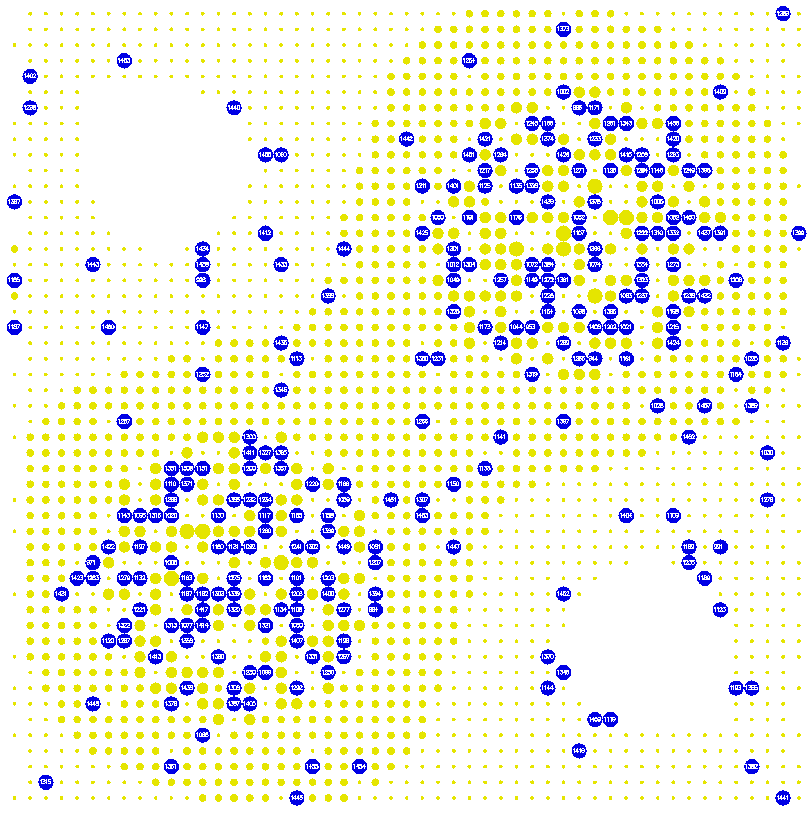
\includegraphics[width=1\textwidth, angle=0]{./fig/background/abs/sugarscape_normal.png}
			\caption{\textit{Animation II-2}: resource growback and infinite agent age.}
			\label{fig:sugarscape_visualisation_normal}
		\end{subfigure}
		
		&
    	
		\begin{subfigure}[b]{0.4\textwidth}
			\centering
			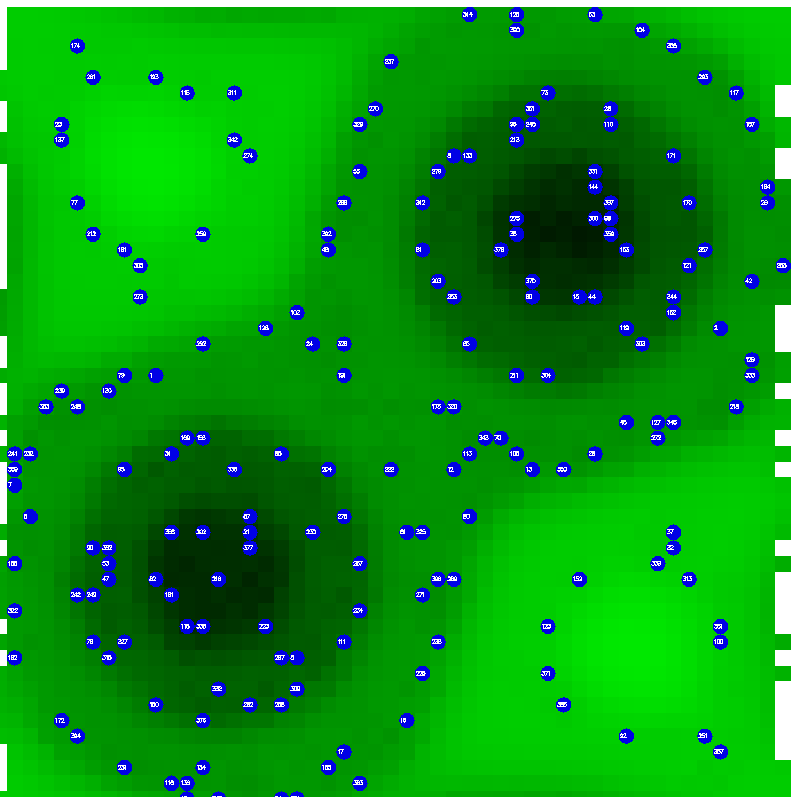
\includegraphics[width=1\textwidth, angle=0]{./fig/background/abs/sugarscape_pollution.png}
			\caption{\textit{Animation II-8}: active pollution with diffusion.}
			\label{fig:sugarscape_visualisation_pollution}
		\end{subfigure}
	\end{tabular}

	
	\begin{tabular}{c c}
		\begin{subfigure}[b]{0.4\textwidth}
			\centering
			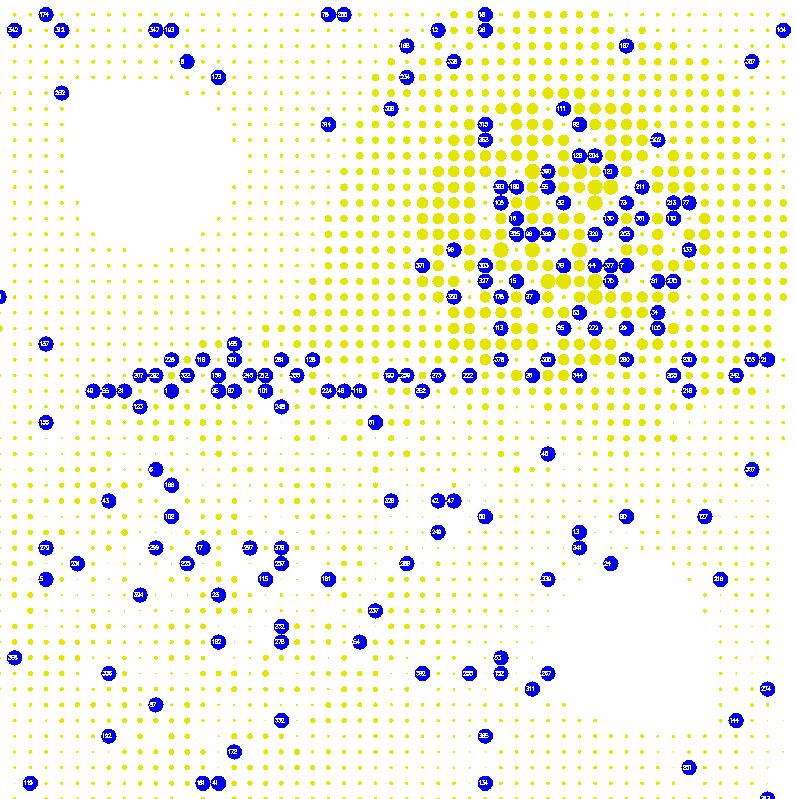
\includegraphics[width=1\textwidth, angle=0]{./fig/background/abs/sugarscape_seasons.png}
			\caption{\textit{Animation II-7}: seasons, agents trying to migrate.}
			\label{fig:sugarscape_visualisation_seasons}
		\end{subfigure}	
		
		& 
		
		\begin{subfigure}[b]{0.4\textwidth}
			\centering
			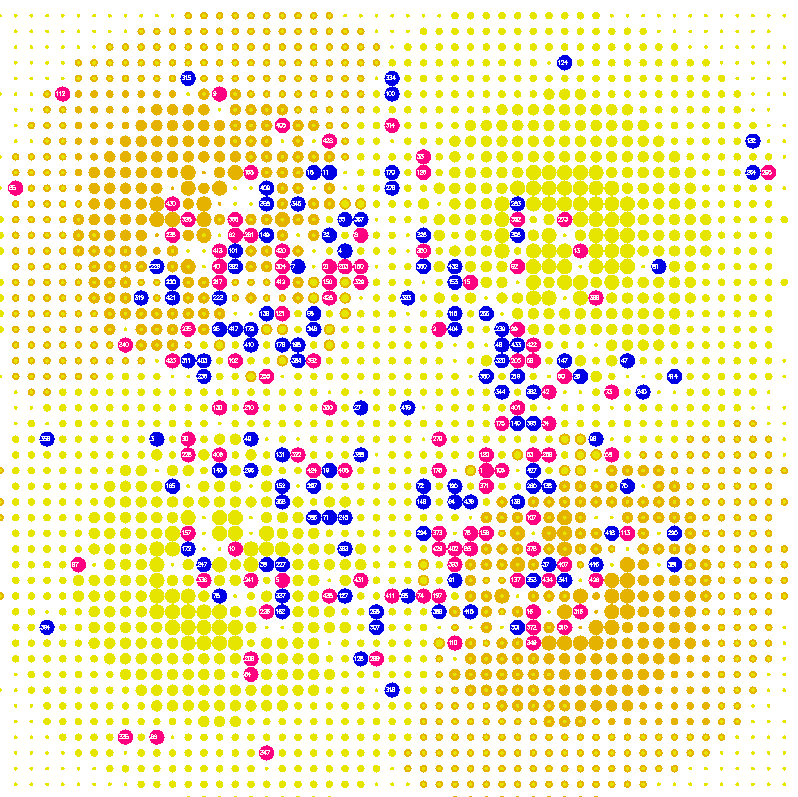
\includegraphics[width=1\textwidth, angle=0]{./fig/background/abs/sugarscape_trading_mating.png}
			\caption{\textit{Figure IV-14}: trading, mating and finite life spans.}
			\label{fig:sugarscape_visualisation_trading_mating}
		\end{subfigure}
	\end{tabular}
	
	\caption{Visualisation of the Sugarscape implementation (see Chapter \ref{sec:eventdriven_implementation}). The naming of the respective \textit{Animation} and \textit{Figure} is taken from \cite{epstein_growing_1996}.} 
	\label{fig:sugarscape_visualisation}
\end{center}
\end{figure}